\begin{pr}$ $
\begin{enumerate}[(a)]
\item $\begin{array}{|c|c|c|c|c|}\hline
A\setminus B&ll&lr&rl&rr\\\hline
L&u_1&u_1&u_2&u_2\\\hline
R&u_3&u_1&u_3&u_1\\\hline
\end{array}$.
\item The saddle points are $(L, lr), (R, lr)$.
\item $v(G_1)=\min(u_1, u_2)=u_1, v(G_2)=\min(u_3, u_1)=u_1$.\\
$\then v(G)=\max(v(G_1), v(G_2))=u_1$.\\
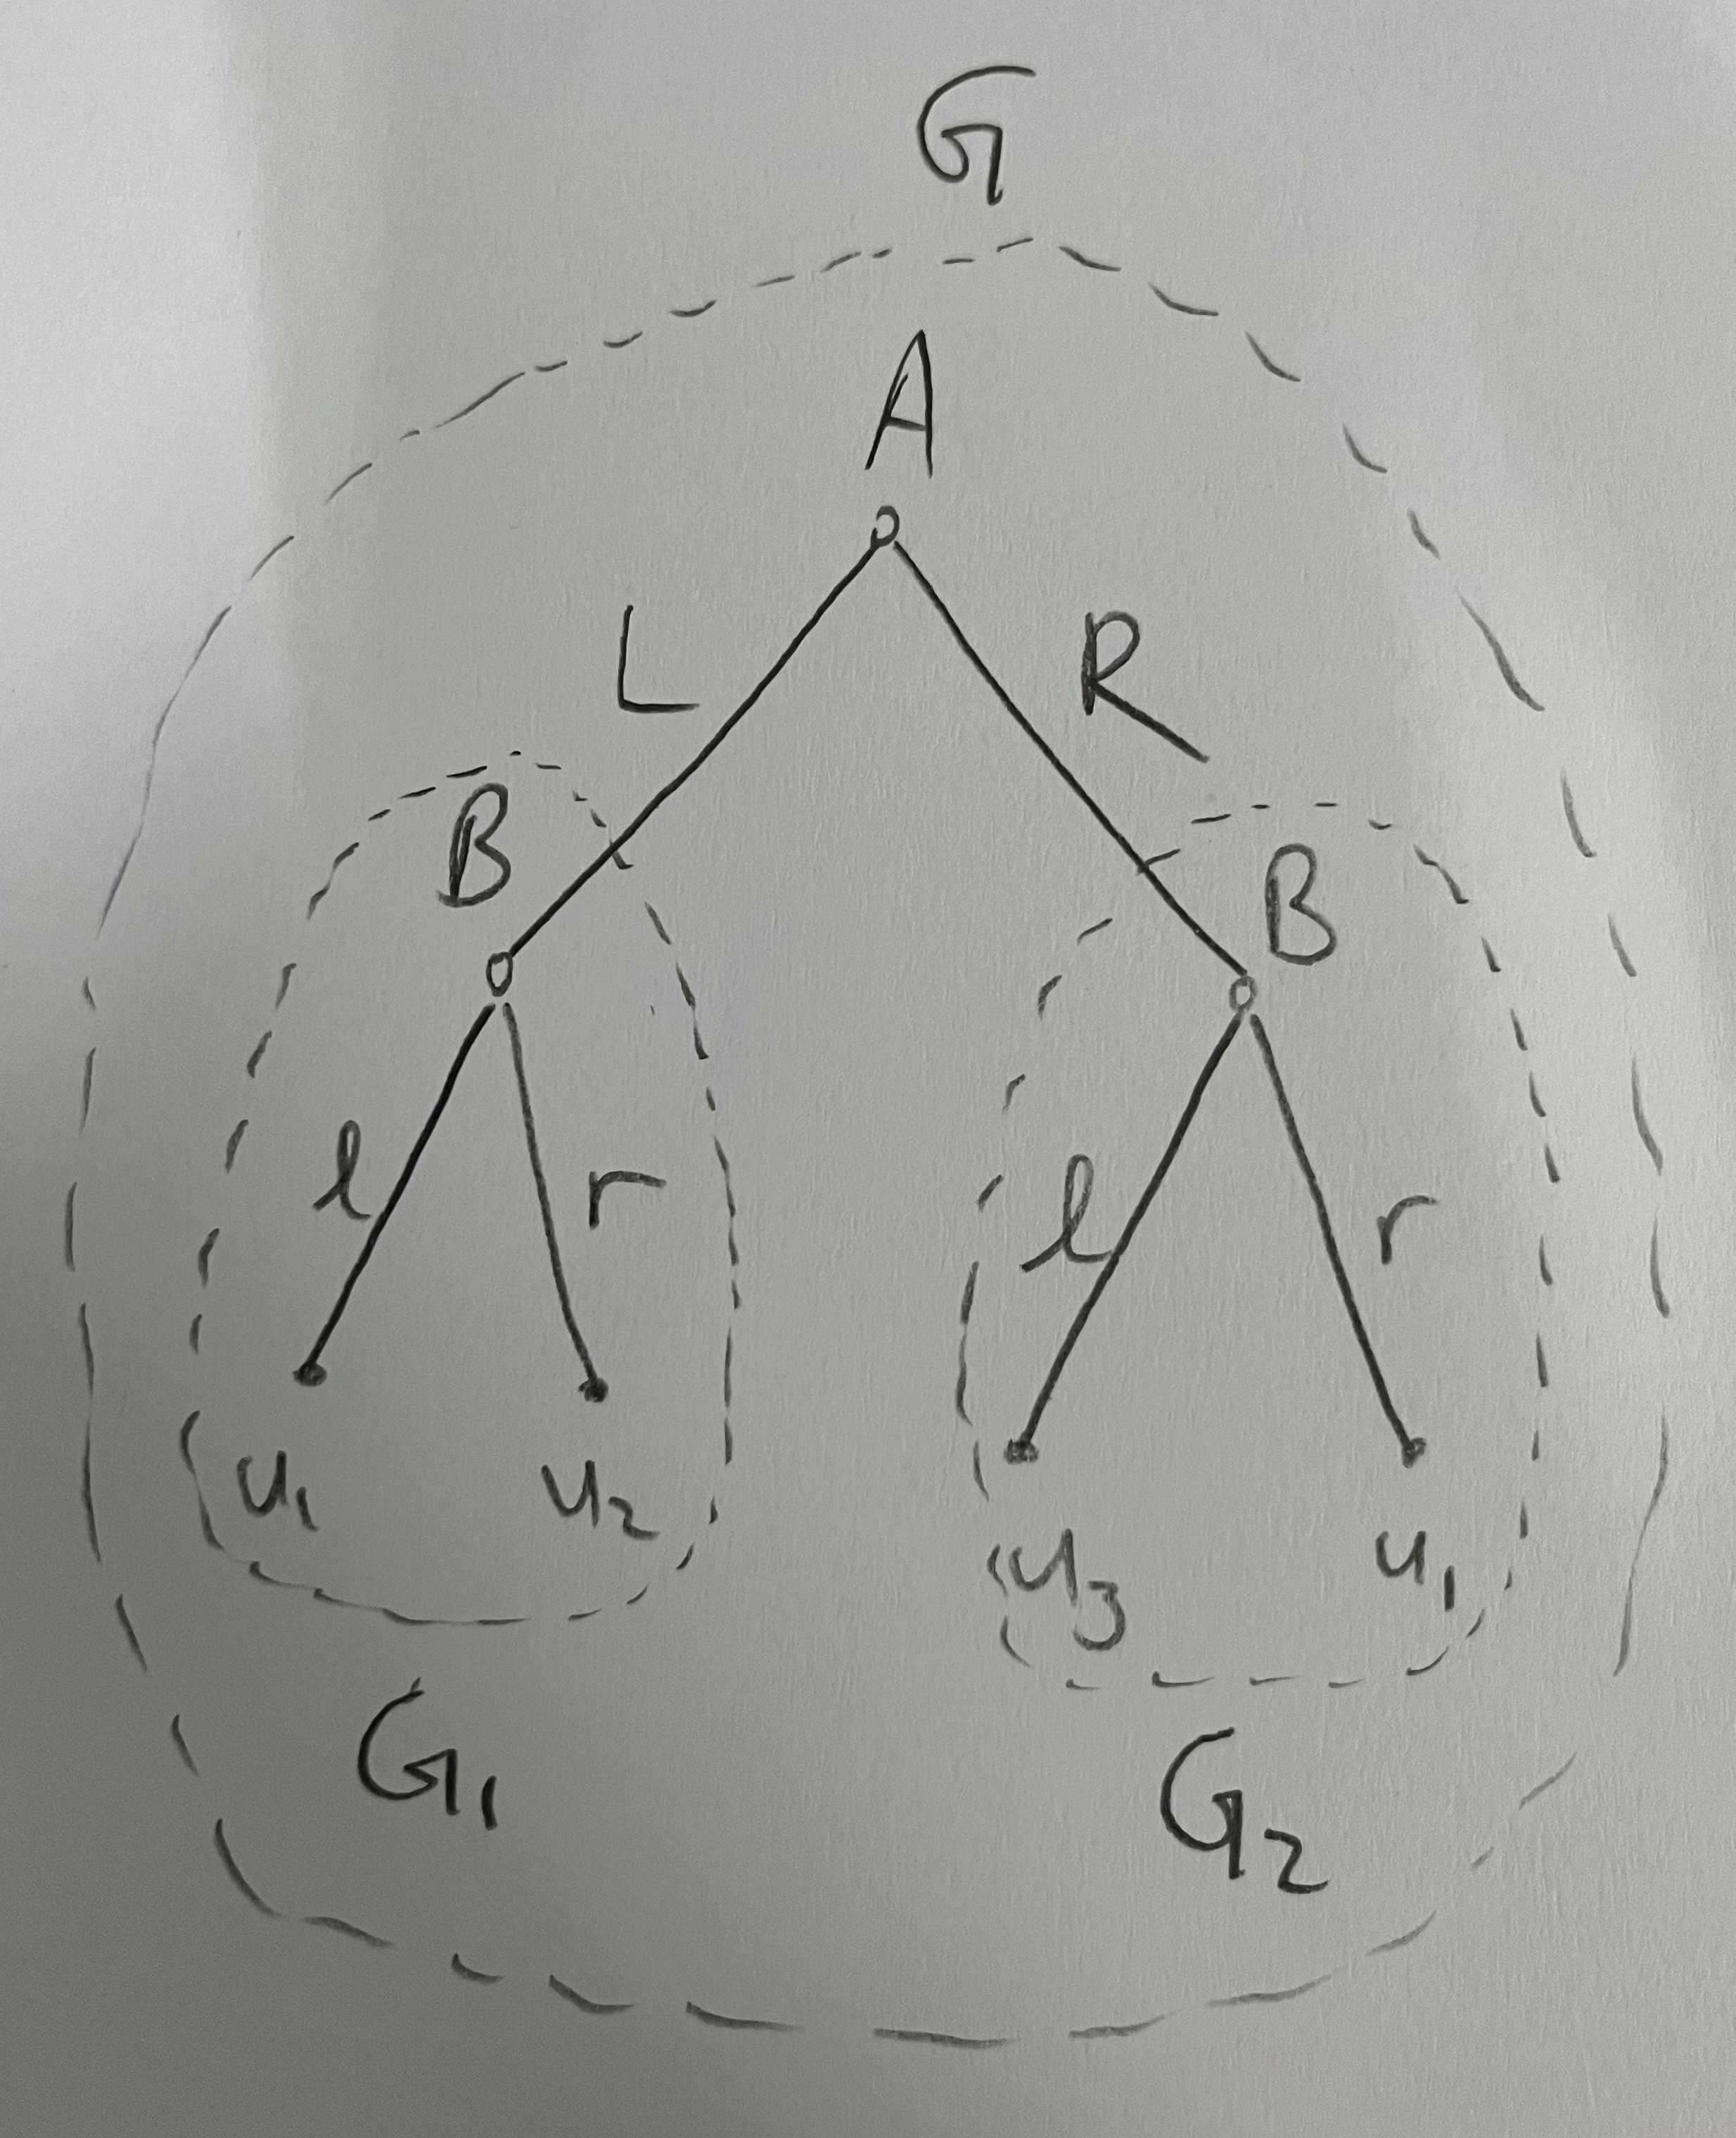
\includegraphics[width=5.5cm]{p1.JPG}
\end{enumerate}
\end{pr}
